\documentclass{echw}

\title{Tutorial A11\\Permutations and Combinations}
\author{Eytan Chong}
\date{2024-08-02}

\begin{document}
    \problem{}
        In a particular country, the alphabet contains 25 letters. A car registration number consists of two different letters of the alphabet followed by an integer $n$ such that $100 \leq n \leq 999$. Find the number of possible car registration numbers.

    \solution
        Note that the number of possible $n$ is $999 - 100 + 1 = 900$. Hence, the number of possible car registration numbers is given by $\comb{25}{2} \cdot 900 = \boxed{540 000}$.

    \problem{}
        A girl wishes to phone a friend but cannot remember the exact number. She knows that it is a five-digit number that is even, and that it consists of the digits 2, 3, 4, 5, and 6 in some order. Using this information, find the greatest number of wrong telephone numbers she could try.

    \solution
        Since the number is odd, there are only 3 possibilities for the last digit. Hence, the maximum wrong numbers she could try is $3 \cdot 4! - 1 = \boxed{71}$.

    \problem{}
        How many ways are there to select a committee of
        \begin{enumerate}
            \item 3 students
            \item 5 students
        \end{enumerate}
        out of a group of 8 students?

    \solution
        \part
            There are $\comb{8}{3} = \boxed{56}$ ways.
        
        \part
            There are $\comb{8}{5} = \boxed{56}$ ways.

    \problem{}
        How many ways are there for 2 men, 2 women and 2 children to sit a round table?

    \solution
        Since the men, women and children are all distinct, there are $(2 + 2 + 2 - 1)! =\boxed{120}$ ways.

    \problem{}
        Find the number of different arrangements of the eight letters of the word NONSENSE if
        \begin{enumerate}
            \item there is no restriction on the arrangement,
            \item the two letters E are together,
            \item the two letters E are not together,
            \item the letters N are all separated,
            \item only two of the letters N are together.
        \end{enumerate}

    \solution
        \part
            Note that N, S and E are repeated 3, 2, and 2 times respectively. Thus, the total number of arrangements is given by $\dfrac{8!}{3! \, 2! \, 2!} = \boxed{1680}$.

        \part
            Consider the two E's as one unit. Altogether, there are 7 units. Hence, the required number of arrangements is given by $\dfrac{7!}{3! \, 2!} = \boxed{420}$.

        \part
            From part (a) and part (b), the required number of arrangements is given by $1680 - 420 = \boxed{1260}$.

        \part
            There are $\dfrac{5!}{2! \, 2!}$ ways to arrange the non-N letters, and $\comb{6}{3}$ ways to slot in the 3 N's into the 6 gaps in between the non-N letters. Thus, the required number of arrangements is given by $\dfrac{5!}{2! \, 2!} \cdot \comb{6}{3} = \boxed{600}$.

        \part
            Consider the three N's as one unit. Altogether there are 6 units. Hence, the number of arrangements where all 3 N's are together is given by $\dfrac{6!}{2! \, 2!} = 180$. 
            
            Thus, from parts (a) and (d), the required number of arrangements is given by $1680 - 600 - 180 = \boxed{900}$.

    \problem{}
        Find the number of teams of 11 that can be select from a group of 15 players
        \begin{enumerate}
            \item if there is no restriction on choice,
            \item if the youngest two players and at most one of the oldest two players are to be included.
        \end{enumerate}

    \solution
        \part
            The number of teams is given by $\comb{15}{11} = \boxed{1365}$.
        
        \part
            Given that the youngest two players are always included, we are effectively finding the number of teams of 9 from a group of 13 players with the restriction that at most one of the oldest two players are to be included.

            Disregarding the restriction, the total number of teams is given by $\comb{13}{9} = 715$.

            Consider now that number of teams where both of the 2 oldest players are included. This is given by $\comb{11}{7} = 330$.

            Thus, the required number of teams is $715 - 330 = \boxed{385}$.

    \problem{}
        A ten-digit number is formed by writing down the digits 0, 1, $\ldots,$ 9 in some order. No number is allowed to start with 0. Find how many such numbers are
        \begin{enumerate}
            \item odd,
            \item less than 2 500 000 000.
        \end{enumerate}

    \solution
        \part
            Since the number is odd, there are 5 possibilities for the last digit. Furthermore, since no number is allowed to start with 0, there are $10 - 2 = 8$ possibilities for the first digit. The remaining 8 digits are free. Hence, the required number of numbers is $5 \cdot 8 \cdot 8! = \boxed{1612800}$.

        \part
            \case{1}{Number starts with 1.} Since there are no further restrictions, the number of valid numbers in this case is $9!$.

            \case{2}{Number starts with 2.} Given the restriction that the number be less than 2 500 000 000, the second digit must be strictly less than 5, thus giving 4 possibilities for the second digit. The remaining 8 digits are free, for a total number of valid numbers of $4 \cdot 8!$.

            Thus, the required number of numbers is $9! + 4 \cdot 8! = \boxed{524160}$.

    \problem{}
        Eleven cards each bear a single letter, and together, they can be made to spell the word ``EXAMINATION''.
        \begin{enumerate}
            \item Three cards are selected from the eleven cards, and the order of selection is not relevant. Find how many possible selections can be made
            \begin{enumerate}
                \item if the three cards all bear different letters,
                \item if two of the three cards bear the same letter.
            \end{enumerate}
            \item Two cards bearing the letter N have been taken away. Find the number of different arrangements for the remaining cards that can be made with no two adjacent letters the same.
        \end{enumerate}

    \solution
        \part
            \subpart

                Observe that there are 8 distinct letters in ``EXAMINATION''. Hence, the number of possible selections is $\comb{8}{3} = \boxed{56}$.

            \subpart

                Note that there are 3 letters that appear twice in ``EXAMINATION''. Hence, the number of possible selections is given by $\comb{3}{1} \cdot  \comb{7}{1} = \boxed{21}$.

        \part
            Note that there are now 2 letters that appear twice, namely A and I. Hence, the total number of possible arrangements is $\dfrac{9!}{2! \, 2!}$.

            Consider ``AA'' and ``II'' as one unit each. Altogether, there are 7 units. The number of arrangements with two pairs of adjacent letters that are the same is hence given by $7!$. 
            
            Consider ``AA'' as one unit, and suppose the two I's are not adjacent to each other. Observe that the non-I letters comprise 6 units, hence giving $6!$ ways of arranging them. Also observe that there are $\comb{7}{2}$ ways to slot in the two I's (which guarantee that they are not adjacent to each other). There are hence $6! \cdot \comb{7}{2}$ possible arrangements in this case. A similar argument follows for the case where the two I's are adjacent but the A's are not.

            From the above discussion, it follows that the required number of arrangements is given by $\dfrac{9!}{2! \, 2!} - 7! - 2 \cdot 6! \cdot \comb{7}{2} = \boxed{55440}$.

    \problem{}
        Find how many three-letter code words can be formed from the letters of the word:
        \begin{enumerate}
            \item PEAR.
            \item APPLE.
            \item BANANA.
        \end{enumerate}

    \solution
        \part
            Since all 4 letters are distinct, the number of code-words is given by $\perm{4}{3} = \boxed{24}$.

        \part
            Tally of letters: 2 `P', 1 `A', 1 `L', 1 `E' (5 letters, 4 distinct).

            \case{1}{All letters distinct.} Since there are 4 distinct letters, the number of code-words in this case is $\perm{4}{3} = 24$.

            \case{2}{2 letters the same, 1 different.} Note that `P' is the only letter repeated more than once. Reserving two spaces for `P' leaves one space left for three remaining letters. Hence, there are $\comb{1}{1} \cdot \comb{3}{1} = 3$ different combinations that can be formed, with $\dfrac{3!}{2!} = 3$ ways to arrange each combination. Hence, the number of code-words in this case is $3 \cdot 3 = 9$.

            Thus, the total number of code-words is $24 + 9 = \boxed{33}$.

        \part
            Tally of letters: 3 `A', 2 `N', 1 `B' (6 letters, 3 distinct).

            \case{1}{All letters distinct.} Since there are only 3 distinct letters, the number of code-words in this case is $\perm{3}{3} = 6$.

            \case{2}{2 letters the same, 1 different.} Observe that both `A' and `N' are repeated more than once. Reserving 2 spaces for either letter leaves one space left for the two remaining letters. Hence, there are $\comb{2}{1} \cdot \comb{2}{1} = 4$ different combinations that can be formed, with $\dfrac{3!}{2!} = 3$ ways to arrange each combination. Hence, the number of code-words in this case is $4 \cdot 3 = 12$.

            \case{3}{All letters the same.} Observe that `A' is the only letter repeated thrice. Hence, the number of code-words in this case is 1.

            Altogether, the total number of code-words is $6 + 12 + 1 = \boxed{19}$.

    \problem{}
        A group of diplomats is to be chosen to represent three islands, $K$, $L$ and $M$. The group is to consist of 8 diplomats and is chosen from a set of 12 diplomats consisting of 3 from $K$, 4 from $L$ and 5 from $M$. Find the number of ways in which the group can be chosen if it includes
        \begin{enumerate}
            \item 2 diplomats from $K$, 3 from $L$ and 3 from $M$,
            \item diplomats from $L$ and $M$ only,
            \item at least 4 diplomats from $M$,
            \item at least 1 diplomat from each island.
        \end{enumerate}

    \solution
        \part
            Note that there are $\comb{3}{2}$ ways to select 2 diplomats from $K$, $\comb{4}{3}$ ways to select 3 diplomats from $L$, and $\comb{5}{3}$ ways to select 3 diplomats from $M$. Thus, the number of possible groups is given by $\comb{3}{2} \cdot \comb{4}{3} \cdot \comb{5}{3} = \boxed{120}$.

        \part
            There are a total of 9 diplomats from $L$ and $M$. Hence, the number of possible groups is $\comb{9}{8} = \boxed{9}$.

        \part
            \case{1}{4 diplomats from $M$.} Note that there are $\comb{5}{4}$ combinations for the 4 diplomats from $M$. Furthermore, since $M$ contributes 4 diplomats, $K$ and $L$ must contribute the other 4 diplomats. Since $K$ and $L$ have a total of 7 diplomats, this gives a total of $\comb{5}{4} \cdot \comb{7}{4}$ possibilities.

            \case{2}{5 diplomats from $M$.} Since $M$ has 5 diplomats, there is only one way for $M$ to send 5 diplomats (all of them have to be chosen). Meanwhile, $K$ and $L$ must contribute the other 3 diplomats from a pool of 7. This gives a total of $\comb{7}{3}$ possibilities.

            Altogether, there are $\comb{5}{4} \cdot \comb{7}{4} + \comb{7}{3} = \boxed{210}$ total possibilities.

        \part
            Observe that $K$ and $M$ have a total of 8 diplomats. Hence, there is only one possibility where the group only consists of diplomats from $K$ and $M$.

            Since $K$ and $L$ have a total of 7 diplomats, it is impossible for the group to only come from $K$ and $L$.

            From part (b), we know that there are 9 ways where the group consists only of diplomats from $L$ and $M$.

            Note that there are a total of $\comb{12}{8}$ possible ways to choose the group.

            Altogether, the required number of possibilities is given by $\comb{12}{8} - 9 - 1 = \boxed{485}$.

    \problem{}
        Alisa and Bruce won a hamper at a competition. The hamper comprises 9 different items.
        \begin{enumerate}
            \item How many ways can the 9 items be divided among Alisa and Bruce if each of them gets at least one item each?
            \item How many ways can a set of 3 or more items be selected from the 9 items?
        \end{enumerate}

    \solution
        \part
            Note that the total number of ways to distribute the items is given by $2^9 = 512$. Also note that the only way either of them does not receive an item is when the other party gets all the items. This can only occur twice (once when Alisa receives nothing, and once when Bruce receives nothing). Thus, the number of ways where both of them gets at least one item each is $512 - 2 = \boxed{510}$.

        \part
            Observe that the number of ways to choose a set of $n$ items from the original 9 is given by $\comb{9}{n}$. Hence, the required number of ways is given by $512 - (\comb{9}{0} + \comb{9}{1} + \comb{9}{2}) = \boxed{466}$.

    \problem{}
        In how many ways can 12 different books be distributed among students A, B, C and D
        \begin{enumerate}
            \item if A gets 5, B gets 4, C gets 2 and D gets 1?
            \item if each student gets 3 books each?
        \end{enumerate}

    \solution
        \part
            At the start, A gets to pick 5 books from the 12 available books. There are $\comb{12}{5}$ ways to do so. Next, B gets to pick 4 books from the $12 - 5 = 7$ remaining books. There are $\comb{7}{4}$ ways to do so. Similarly, there are $\comb{3}{2}$ ways for C to pick his book, and $\comb{1}{1}$ ways for D to pick his. Hence, there are a total of $\comb{12}{5} \cdot \comb{7}{4} \cdot \comb{3}{2} \cdot \comb{1}{1} = \boxed{83160}$ ways for the 12 books to be distributed.

        \part
            Following a similar argument as in part (a), the number of ways the 12 books can be distributed is given by $\comb{12}{3} \cdot \comb{9}{3} \cdot \comb{6}{3} \cdot \comb{3}{3} = \boxed{369600}$.

    \problem{}
        3 men, 2 women and 2 children are arranged to sit around a round table with 7 non-distinguishable seats. Find the number of ways if
        \begin{enumerate}
            \item \begin{enumerate}
                \item the 3 men are to be together,
                \item the 3 men are to be together, and the seats are numbered,
            \end{enumerate}
            \item no 2 men are to be adjacent to each other,
            \item only 2 men are adjacent to each other.
        \end{enumerate}

    \solution
        \part
            \subpart

                Consider the 3 men as one unit. Altogether, there are a total of 5 units, which gives a total of $(5 - 1)! = 4!$ ways for the 5 units to be arranged around the table. Since there are $3!$ ways to arrange the men, there are a total of $4! \cdot 3! = \boxed{144}$ arrangements.

            \subpart

                Since there are a total of 7 distinguishable seats, the total number of arrangements is 7 times that of the number of arrangements with non-distinguishable seats. From part (a), this gives $144 \cdot 7 = \boxed{1008}$ total arrangements.

        \part
            Observe that there is only one possible layout for no 2 men to be adjacent to each other (as shown in the diagram below). Since there are $4!$ ways to arrange the non-men, and $3!$ ways to arrange the men, there are a total of $4! \cdot 3! = \boxed{144}$ arrangements.

            \begin{center}
                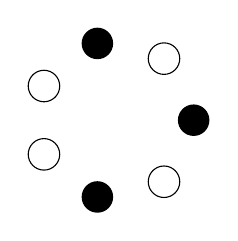
\begin{tikzpicture}
                    \draw ({cos(360/7)}, {sin(360/7)}) circle (0.2cm);
                    \fill ({cos(360*2/7)}, {sin(360*2/7)}) circle (0.2cm);
                    \draw ({cos(360*3/7)}, {sin(360*3/7)}) circle (0.2cm);
                    \draw ({cos(360*4/7)}, {sin(360*4/7)}) circle (0.2cm);
                    \fill ({cos(360*5/7)}, {sin(360*5/7)}) circle (0.2cm);
                    \draw ({cos(360*6/7)}, {sin(360*6/7)}) circle (0.2cm);
                    \fill ({cos(360*7/7)}, {sin(360*7/7)}) circle (0.2cm);
                \end{tikzpicture}
            \end{center}

        \part
            Observe that there are 3 possible layouts for only 2 men to be adjacent to each other (as shown in the diagram below). Since there are $4!$ ways to arrange the non-men, and $3!$ ways to arrange the men, there are a total of $3 \cdot 4! \cdot 3! = \boxed{432}$ arrangements.

            \begin{center}
                \begin{tikzpicture}
                    \fill ({cos(360/7)}, {sin(360/7)}) circle (0.2cm);
                    \draw ({cos(360*2/7)}, {sin(360*2/7)}) circle (0.2cm);
                    \fill[plotRed] ({cos(360*3/7)}, {sin(360*3/7)}) circle (0.2cm);
                    \fill[plotRed] ({cos(360*4/7)}, {sin(360*4/7)}) circle (0.2cm);
                    \fill[plotRed] ({cos(360*5/7)}, {sin(360*5/7)}) circle (0.2cm);
                    \draw ({cos(360*6/7)}, {sin(360*6/7)}) circle (0.2cm);
                    \fill ({cos(360*7/7)}, {sin(360*7/7)}) circle (0.2cm);
                \end{tikzpicture}
            \end{center}
            

    \problem{}
        Find the number of ways for 4 men and 4 boys to be seated alternately if they sit
        \begin{enumerate}
            \item in a row,
            \item at a round table.
        \end{enumerate}

    \solution
        \part
            Note that there are 2 possible layouts: one where a man sits at the start of the row, and one where a boy sits at the start of the row. Since there are $4!$ ways to arrange both the men and boys, there are a total of $2 \cdot 4! \cdot 4! = \boxed{1152}$ arrangements.
        
        \part
            Given the rotational symmetry of the circle, there is now only one possible layout. Fixing one man, there are $3!$ ways to arrange the other men and $4!$ ways to arrange the boys, giving a total of $3! \cdot 4! = \boxed{144}$ arrangements.

    \problem{}
        A rectangular shed, with a door at each end, contains ten fixed concrete bases marked $A$, $B$, $C$, $\ldots,$ $J$, five on each side (see diagram). Ten canisters, each containing a different chemical, are placed with one canister on each base. In how many ways can the canisters be placed on the bases?

        \begin{center}
            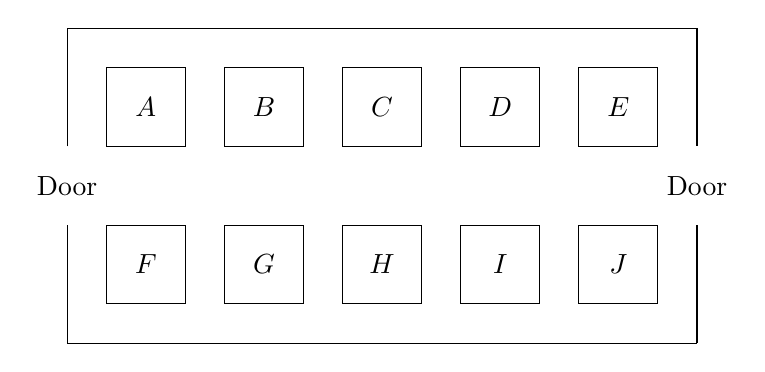
\begin{tikzpicture}
                \draw (-4, 0.5) -- (-4, 2);
                \draw (-4, 2) -- (4, 2);
                \draw (4, 2) -- (4, 0.5);

                \draw (-4, -0.5) -- (-4, -2);
                \draw (-4, -2) -- (4, -2);
                \draw (4, -2) -- (4, -0.5);

                \draw (-0.5, 0.5) rectangle (0.5, 1.5);
                \draw (-2, 0.5) rectangle (-1, 1.5);
                \draw (-3.5, 0.5) rectangle (-2.5, 1.5);
                \draw (2, 0.5) rectangle (1, 1.5);
                \draw (3.5, 0.5) rectangle (2.5, 1.5);

                \draw (-0.5, -0.5) rectangle (0.5, -1.5);
                \draw (-2, -0.5) rectangle (-1, -1.5);
                \draw (-3.5, -0.5) rectangle (-2.5, -1.5);
                \draw (2, -0.5) rectangle (1, -1.5);
                \draw (3.5, -0.5) rectangle (2.5, -1.5);

                \node at (-3, 1) {$A$};
                \node at (-1.5, 1) {$B$};
                \node at (0, 1) {$C$};
                \node at (1.5, 1) {$D$};
                \node at (3, 1) {$E$};

                \node at (-3, -1) {$F$};
                \node at (-1.5, -1) {$G$};
                \node at (0, -1) {$H$};
                \node at (1.5, -1) {$I$};
                \node at (3, -1) {$J$};

                \node at (4, 0) {Door};
                \node at (-4, 0) {Door};
            \end{tikzpicture}
        \end{center}

        Find the number of ways in which the canisters can be placed
        \begin{enumerate}
            \item if 2 particular canisters must not be placed on any of the 4 bases $A$, $E$, $F$ and $J$ next to a door,
            \item if 2 particular canisters must not be placed next to each other on the same side.
        \end{enumerate}

    \solution
        There are $10! = \boxed{3628800}$ ways to place the canisters on the bases.

        \part
            Observe that there are $\perm{6}{2}$ possible placements for the two particular canisters. Since the other 8 canisters have no restrictions, the total number of ways to place the canisters is given by $\perm{6}{2} \cdot 8! = \boxed{1209600}$.
            
        \part
            Consider the number of ways the two particular canisters can be placed adjacently. There are $2 \cdot (5-1) = 8$ possible arrangements per side, giving a total of $2 \cdot 8 = 16$ possible arrangements. Since the other 8 canisters have no restrictions, the total number of ways to place the canisters is given by $16 \cdot 8! = 645120$. The required number of ways is thus given by $3628800 - 645120 = \boxed{2983680}$.
\end{document}